% -----------------------------------------------------------------
% Vorlage fuer Ausarbeitungen von
% Bachelor- und Masterarbeiten am ISS
% 
% Template for written reports or master theses at the ISS
% 
% For use with compilers pdflatex or latex->dvi2ps->ps2pdf.
%
% -----------------------------------------------------------------
% README, STUDENT USERS:
% We highly appreciate students using this template _AS IS_,period. 
% The document provides adjustable document preferences, 
% student information settings and typography definitions. Look for
% code delimited by *** ***
%
% The short explanation: it's the ISS common standard and 
% 	it's battle tested.
% The long explanation: 
%	We do not want you to go through the document and tweak the 
%	package options, layout parameters and line skips here and 
%	there and waste hours. We are providing this template such 
%	that you can fully concentrate on filling in the much more 
%	important _contents_ of your thesis.
%
% If you have serious needs on extra packages or design 
% modifications, talk to your supervisor _before_ modifying 
% the template.
% Similarly, we're happy if you give your supervisor a hint on any 
% errors in this template.
%
% -----------------------------------------------------------------
% History:
% Jan Scheuing,   04.03.2002
% Markus Buehren, 20.12.2004
% last changes:   10.01.2008 (removed unused packages), 
% 		07.08.2009 (added IEEEtran_LSS.bst file)
% 		02.05.2011 removed matriculation number from cover page
% Martin Kreissig, 25.01.2012, all eps/ps parts removed for 
% 				pdflatex to work properly
% Peter Hermannstaedter, 14.08.2012, fusion of versions for 
% 		latex/dvi/ps/pdf and pdflatex, additional comments,
% 		unification of document flags and student options
%
% -----------------------------------------------------------------
% To do: 
% - remove obsolete documentclass options if all our systems 
%	have up-to-date tex distributions
% -----------------------------------------------------------------


\documentclass[12pt,DIV14,BCOR12mm,a4paper,footexclude,headinclude,halfparskip-,twoside,openright,openany,cleardoubleempty,idxtotoc,bibtotoc]{scrreprt} % Koma-Script
%
%
%
% *****************************************************************
% -------------------> document preferences here <-----------------
% *****************************************************************
% Uncomment the settings you like and comment the settings you dont
% like.

% Language: 
% affects generic titles, Figure term, titlepage and bibliography
% (Note:if you switch the language, compile tex and bib >2 times)
\def \doclang{english} 	% For theses/reports in English
%\def \doclang{german} 		% For theses/reports in German

% Hyperref links in the document:
\def \colortype{color} % links with colored text
%\def \colortype{bw} 	% plain links, standard text color (e.g. for print)
%\def \colortype{boxed} % links with colored boxes
% *****************************************************************
%
%
%
% *****************************************************************
% --------------> put student information here <------------------
% *****************************************************************
% Pleas fill in all items denoted by "to be defined (TBD)"
\def \deworktitle{Vergleich von aktuellen Clustering Algorithmen}        % German title/translation
\def \enworktitle{Comparison of State-of-the-art Clustering algorithm}       % English title/translation
\def \tutor{Alexander Bartler}
\def \student{Simon Kamm}
\def \worksubject{Research Thesis s1279}
\def \startdate{22.10.2018}
\def \submission{21.04.2019}
\def \signagedate{21.04.2019}   % Date of signature of declaration on last page
\def \keywords{deep learning, unsupervised learning, clustering, autoencoder, variational autoencoder, kmeans, gaussian mixture model}
\def \abstract{Current "state-of-the-art" clustering algorithms are usually consist of two parts. The first one is a dimensionality reduction (often called feature extraction) part while the second uses the extracted and reduced features and perform clustering on this. In this work, some selecet current "state-of-the-art" clustering models based on different autoencoder models are implemented. A large-scale evaluation for this models is done to check their performance on (more and less) complicated datasets (from 32x32 greayscale images of MNIST \cite{MNIST-Data} to 64x64 rgb images of IMAGENET \cite{imagenet_cvpr09}). Additionallythe effect of different hyperparameter settings is investigated. Hyperparameters are seperated into two kinds of hyperparameters. They are seperated into model-related hyperparameter, which directly influence the model (i.e. size of latentspace) and training-related hyperparameters (i.e. learning rate schedule, batch size, etc.). The procedure will be, that the specific model-related hyperparameters are first optimized based on "basic" training-related hyperparameters. The model-related hyperparameters will then be fixed and the second set of hyperparameters will be varied and their impact on clustering performance will be investigated.
In this work state-of-the-art algorithms will be investigated, implemented and optimized inside a self-programmed framework (in Tensorflow) with comparative model architectures and training procedure. These different models are then evaluated with different hyperparameters on different Datasets.}
% \def \studentID{Matriculation number}  % matriculation number on cover sheet deprecated (2011-05-02)

% *****************************************************************
%
%

\usepackage[latin1]{inputenc}
\usepackage{amsmath}
\usepackage{amsfonts}
\usepackage{ifthen}
\ifthenelse{\equal{\doclang}{german}}{
	\usepackage[ngerman]{babel} %german version!!
	\def \langtitle{\enworktitle}
	%\def \suptitle{\enworktitle}	
}{
	%english version!!
	\def \langtitle{\enworktitle}
	\def \suptitle{\deworktitle}
}
\usepackage{txfonts} % Times-Fonts
\usepackage[T1]{fontenc}
\usepackage{color}
\usepackage[headsepline]{scrpage2} % Headings

\usepackage{graphicx}
\usepackage[format=hang]{caption}       % for hanging captions
\usepackage{subfig}                     % for subfigures
\usepackage{wrapfig}                    % for figures floating in text, alternatively you can use >>floatflt<<
\usepackage{booktabs}

\ifthenelse{\equal{\colortype}{color}}{
	% colored text version:
	\usepackage[colorlinks,linkcolor=blue]{hyperref}
	\newcommand{\bugfix}{\color{white}{\texttt{\symbol{'004}}}} % Bug-Fix Umlaute in Verbatim
}{
	\ifthenelse{\equal{\colortype}{boxed}}{
		% colored box version:
		\usepackage{hyperref}
		\newcommand{\bugfix}{\color{white}{\texttt{\symbol{'004}}}} % Bug-Fix Umlaute in Verbatim
	}{
		% monochrome version:
		\usepackage[hidelinks]{hyperref}
		\newcommand{\bugfix}{\color{white}{\texttt{\symbol{'004}}}} % Bug-Fix Umlaute in Verbatim
	}
}

% Layout and Headings
\pagestyle{scrheadings}
\automark{chapter}
\clearscrheadfoot
\lehead[]{\pagemark~~\headmark}
\rohead[]{\headmark~~\pagemark}
\renewcommand{\chaptermark}[1]{\markboth {\sl \hspace{8mm}#1}{}}
\renewcommand{\sectionmark}[1]{\markright{\sl \thesection~#1\hspace{8mm}}}
\addtolength{\textheight}{15mm}
\parindent0ex
\setlength{\parskip}{5pt plus 2pt minus 1pt}
\renewcommand*{\pnumfont}{\normalfont\slshape} % Seitenzahl geneigt
\renewcommand*{\sectfont}{\bfseries} % Kapitelueberschrift nicht Helvetica

% Settings for PDF document
\pdfstringdef \studentPDF {\student}
\pdfstringdef \worktitlePDF {\langtitle}
\pdfstringdef \worksubjectPDF {\worksubject}
\hypersetup{pdfauthor=\studentPDF, 
	pdftitle=\worktitlePDF,
	pdfsubject=\worksubjectPDF}

% Title page
\titlehead{
	
\includegraphics[width=20mm]{university-logo}
	\hspace{6mm}
	\ifthenelse{\equal{\doclang}{german}}{
		\begin{minipage}[b]{.6\textwidth}
			{\Large Universit\"at Stuttgart } \\
			Institut f\"ur Signalverarbeitung und Systemtheorie\\
			Professor Dr.-Ing. B. Yang \vspace{0pt}
		\end{minipage}
	}{
		\begin{minipage}[b]{.6\textwidth}
			{\Large University of Stuttgart } \\
			Institute for Signal Processing and System Theory\\
			Professor Dr.-Ing. B. Yang \vspace{0pt}
		\end{minipage}
	}
	\hspace{1mm}
	
\includegraphics[width=28mm]{isslogocolor}
}
\subject{\worksubject\vspace*{-5mm}} % Art und Nummer der Arbeit
\title{\Large{\langtitle}}
\author{
	\large
	\ifthenelse{\equal{\doclang}{german}}{
		\begin{tabular}{rp{7cm}}
			\Large 
			Autor:      & \Large \student \vspace*{2mm}\\
			%    Matr.-Nr.:  & \studentID \\
			Ausgabe:    & \startdate \\
			Abgabe:     & \submission \vspace*{3mm}\\
			Betreuer:   & \tutor \vspace*{2mm}\\
			Stichworte: & \keywords
		\end{tabular}
	}{
		\begin{tabular}{rp{7cm}}
			\Large 
			Authors:             & \Large \student \vspace*{2mm}\\
			%    Matr.-Nr.:          & \studentID \\
			Date of work begin: & \startdate \\
			Date of submission: & \submission \vspace*{3mm}\\
			Supervisor:         & \tutor \vspace*{2mm}\\
			Keywords:           & \keywords
		\end{tabular}
	}
	\bugfix
}
\date{}
\publishers{\normalsize
	\begin{minipage}[t]{.9\textwidth}
		\abstract
	\end{minipage}
}

\numberwithin{equation}{chapter} 
\sloppy 

%
%
%
% *****************************************************************
% --------------> put typography definitions here <----------------
% *****************************************************************
% colors
\definecolor{darkblue}{rgb}{0,0,0.4}

% declarations
\newcommand{\matlab}{\textsc{Matlab}\raisebox{1ex}{\tiny{\textregistered}} }
\newcommand{\Z}{\mathbb{Z}}
\newcommand{\N}{\mathbb{N}}
\newcommand{\R}{\mathbb{R}}
\newcommand{\E}{\operatorname{E}}
\newcommand{\e}[1]{\operatorname{e}^{\,#1}}
\newcommand{\op}[1]{\operatorname{#1}}
\newcommand{\smtext}[1]{{\scriptscriptstyle\text{#1}}}

% unknown hyphenation rules
\hyphenation{Im-puls-ant-wort Im-puls-ant-wort-ko-ef-fi-zien-ten
	Pro-gramm-aus-schnitt Mi-kro-fon-sig-nal}
% *****************************************************************
%
%
%
% *****************************************************************
\begin{document}
	
	% title and table of contents
	\maketitle
	\pagenumbering{roman} % roman numbering for table of contents
	\tableofcontents
	\cleardoublepage
	\setcounter{page}{1}
	\pagenumbering{arabic} % arabic numbering for rest of document
	
	% *****************************************************************
	% -------------------> start writing here <------------------------
\chapter{Introduction}
The field of unsupervised learning is a fundamental one in machine learning. Since nearly every novel product is connected, a tremendous amount of data is generated. Neither every single data can be labelled, nor is it possible or desired to save the whole original data, since in most application not all recorded is useful. Therefore, in the area of unsupervised learning, tasks like dimensionality reduction (sometimes also called representation learning) or clustering are important to extract relevant features or/and group similar data together. Those two tasks are directly linked, since state-of-the art clustering methods use as first step a dimensionality reduction to on the one hand reduce the feature space but also extract the relevant features out of the data. Important for these models is, that they still want to perform the decoding step based on latent representations. So the reduced feature space should not just be a good representation for clustering similar data, but also allow a good reconstruction of the original data. Therefore, in most of these works a deep auto-encoder (or a variation of it) is first trained to extract those relevant features but also ensure a good reconstruction of the latent space. Different learning approaches exist to achieve this task. Traditionally, most learning approaches treat feature-selection/representation-learning and clustering separately. However, some novel approaches outperform traditional ones, by combining these two task. In this work, both kind of approaches are represented. Although in all of those works a very good performance (in this case clustering accuracy) and generalizability is claimed, the experiments given in the publications are often limited with respect to datasets and/or variation of hyperparameters. Therefore, in this work, different methods for clustering images are implemented and evaluated inside a self-programmed framework within Tensorflow to allow a fair comparison of those methods.\\
First, a short overview of the theoretical background for deep learning and unsupervised learning is given. Followed by a more specific part about the idea and main algorithms for dimensionality reduction/ representation learning and clustering. Chapter two will explain the working environment which will be further used in this work. The third chapter introduces the used architectures and algorithms, as well as the related hyperparameters of the models. The mentioned algorithms are implemented inside the environment explained in chapter two. Chapter four defines the experimental setup for the evaluation of the models. This chapter introduces the used datasets as well as the investigated hyperparameters. Following this chapter, chapter five discusses and visualizes the results of the experiments. The final chapter 6 summarizes the work and gives a outlook about further possible investigations or steps which can be derived based on this work.

\chapter{Theoretical background}
This chapter gives a short overview about the theoretical basics which are necessary for the following work. First a general overview about deep learning is given with respect to its main critical parts. Then it will go into more detail about unsupervised learning followed by more specific parts about dimensionality reduction and clustering. General it can be said that dimensionality reduction and clustering are specific tasks of unsupervised learning, which is on the other hand a sub domain of deep learning. A graphical overview of the relationship between these mentioned domains is given in figure \ref{fig:Relationship_DL}. 
\begin{figure}[htb!]
	\centering
	\includegraphics[width=0.5\linewidth]{Graphiken/Overview_Deep_Learning}
	\caption{Relationship between deep learning, unsupervised learning, clustering and dimensionality reduction}
	\label{fig:Relationship_DL}
\end{figure}

\section{Deep Learning}
This section will give a rough overview about deep learning, the way deep neural networks actually work and how it is possible to train them. Firstly, the relation between deep learning and machine learning is explained. Then the general structure and behaviour of a neural network is explained and the algorithm for training those networks is introduced. Finally some difficulties in training these networks are named with corresponding solutions.\\
Deep learning is a sub area of machine learning, which is in general a learning-based or data-driven approach to design a processing rule (see figure \ref{fig:ProcessingRule}). The learning of this processing rule is based on examples. So it's obvious that the choice of training samples is crucial for learning a good and generalized processing rule. 
\begin{figure}[htb!]
	\centering
	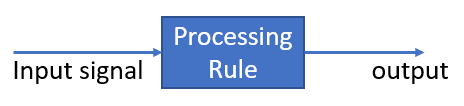
\includegraphics[width=0.5\linewidth]{Graphiken/ProcessingRule}
	\caption{General problem formulation in machine learning}
	\label{fig:ProcessingRule}
\end{figure}
There is one main difference between conventional machine learning and deep learning. While they have in common, that they get input data which is preprocessed depending on the application, in conventional machine learning features are extracted based on a defined rule (\cite{Goodfellow-et-al-2016}). For this task, no theory exists and experience is necessary to choose good and relevant features for the following task, i.e. classification. The classification is done by a classifier, like kNN (k-nearest neighbour) or SVM (Support Vector Machine). In deep learning, there exists just one so-called deep neural network (DNN) for the tasks feature extraction and classification. The DNN learns and adapts the network parameters by a proper loss function. This can be obtained efficiently using the technique of (error) backpropagation (\cite{Goodfellow-et-al-2016}, \cite{Nielsen-Michael}, \cite{DeepLearningDive}, \cite{Bishop}). More details will be given in the following.\\
The learning strategy for DNNs is adapted from the way humans learn to recognize, speak, walk, calculate etc.. Despite deep learning is often seen as a exciting new technology, it can be dated back to the 1940s. Following \cite{Goodfellow-et-al-2016}, there have been three waves of development: In the 1940s-1960s (known as cybernetics), between 1980 and 1990 as connectionism and the current resurgence under the recent name deep learning beginning in 2006. The third wave of development, which is still in progress began with a breakthrough by Geoffrey Hinton. He showed that a special kind of neural network, the so called "Deep Belief Network" could be trained efficiently using a strategy called greedy layer-wise pretraining \cite{Hinton-et-al-2006}.\\
Since this breakthrough, the applications of deep neural networks increases tremendously. Examples for applications of deep neural networks nowadays are recommender systems, automatic speech recognition, text to speech translation, image recognition and/or segmentation and a lot more \cite{DeepLearningDive}. For a special task the networks are typically adjusted and the architecture is adapted. Therefore a lot of variation of deep neural networks exists nowadays, examples mentioned in \cite{Nielsen-Michael} are convolutional neural networks (CNNs), recurrent neural networks (RNNs), deep belief nets (DBNs).\\
In the following, the architecture of a feedforward neural network is exemplary showed, since "deep feedforward networks, also called feedforward neural networks or multilayer perceptrons (MLPs), are the quintessential deep learning models" \cite{Goodfellow-et-al-2016}. The naming "feedforward" comes from behaviour, that information flows in forward direction through the network, so from the input signal to the output. There is no feedback connection inside the model. These feedforward neural networks consists of multiple layers stacked together to a network. Each layer consists of many neurons. Figure \ref{fig:SingleNeuron} shows one single neuron.
\begin{figure}[htb!]
	\centering
	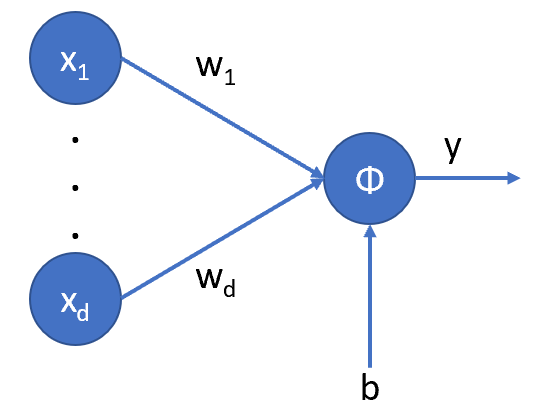
\includegraphics[width=0.3\linewidth]{Graphiken/SingleNeuron}
	\caption{Single Neuron in a feedforward neural network}
	\label{fig:SingleNeuron}
\end{figure}
In equation \ref{eq:singleneuron}, the output $y$ of a single neuron is given, with $\phi$ is the (typically non-linear) activation function of the activation $a$ which is an affine function in $\underline{x}$. $\underline{x}$ is the input vector, or the 2-d input image or 3-d input tensor. The trainable parameters of the neuron are the weights $\underline{w}$ and the bias $b$.
\begin{align}
	a = \underline{w}{^T}*\underline{x}+b\\
	y = \phi(a) \label{eq:singleneuron}
\end{align}
A layer of neurons, as drawn in figure \ref{fig:Layer_of_neurons}, consists of $c$ neurons, which are connected with the input and output. The neurons in the same are not interconnected between each other. Depending on the network structure, the connections to the input and output varies. For a dense (or fully connected) layer, each input $x_{j}$ is connected to each neuron $i$.
\begin{figure}[htb!]
	\centering
	\subfloat[Layer of Neurons\label{fig:NeuronsLayer}]{%			
		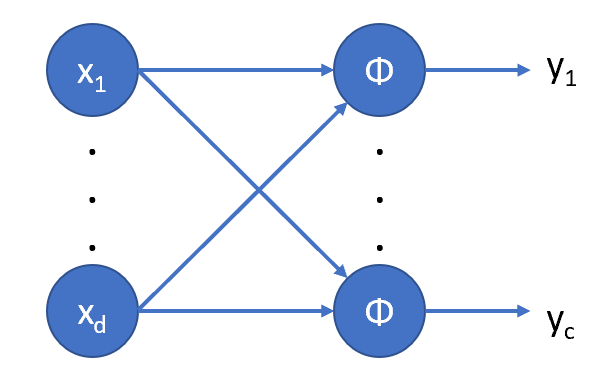
\includegraphics[width=0.45\linewidth]{Graphiken/NeuronsLayer}}
	\qquad
	\subfloat[Layer of Neurons compressed visualization\label{fig:NeuronsLayer_Matrix}]{%			
		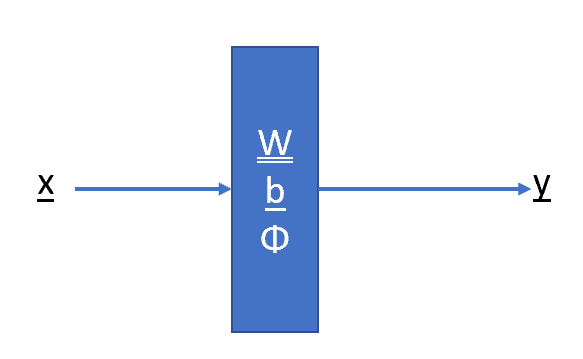
\includegraphics[width=0.45\linewidth]{Graphiken/NeuronsLayer_Matrix}}
	\caption{Layer of Neurons in feedforward neural network}
	\label{fig:Layer_of_neurons}
\end{figure}
After defining one layer, a layer can be followed by another and so on. The overall length of the chaing gives the depth of the model. From this terminology, the name deep learning arose. The first layer of a network is the "input layer", while the last one is the "output layer". Those two layers have fixed sizes, since the input and the output data of a network has a defined size. All layers between them are called hidden layers. These layers are called hidden since they are neither visible to the inputs nor the outputs. Different to the the input and output layers, their size is not fixed. They are generally used to form a \textit{bottleneck}, forcing the network to make a simple model of the system with the ability to generalise to previously unseen patterns (test data) \cite{Michie-et-al-1994}. By using non-linear activation functions, such as softmax (equation \ref{eq:softmax}) or rectifier linear unit (ReLU) (equation \ref{eq:ReLU}), it can be shown that already a "two-layer MLP can approximate an arbitrary continous mapping arbitrarily closely if there is no limit to the number of hidden nodes" \cite{Michie-et-al-1994}. This property of neural networks is also known as universal function approximation.
\begin{align}
	\phi_{i}(\underline{a}) = \frac{e^{a_{i}}}{\sum_{j=1}^{c}e^{a_{j}}} \label{eq:softmax}\\
	\phi_{i}(a_{i}) = \begin{cases} 1 & a_{i} > 0\\0 & a_{i} \leq 0\\ \end{cases} \label{eq:ReLU}
\end{align}
If linear activation functions would be used, the overall network, independent on the depth of the network, will overall be just a linear transformation of the input data, so only linear solvable problems could be solved. This shows the importance for choosing non-linear activation functions.\\
For training a neural network, a loss function based on the training data has to be defined, which has to be minimized, with respect to the network parameters. 
Overall, the training task for a neural network is to minimize the cost function $L(\underline{\theta})$ on the training data as given in equation \ref{eq:CostFunction} with $\iota(\underline{x}(n),\underline{y}(n);\underline{\theta})$ is an arbitrary loss function where $\underline{y}$ is the target output of the network and $\underline{x}$ is the input of the network. The cost function denotes the total loss over all $N$ samples.
\begin{align}
	\underset{\underline{\theta}}\min L(\underline{\theta}) = \frac{1}{N}\sum_{n=1}^{N}\iota(\underline{x}(n),\underline{y}(n);\underline{\theta})  \label{eq:CostFunction}
\end{align}
The loss function is depending on the task. For regression, a typical loss function is the $l_{2}$-loss, where $l_{2}$-Norm of the error is used. The error is the difference between the target output $\underline{y}$ and the output of the neural network, $f(\underline{x};\underline{\theta})$. This loss function is given in equation \ref{eq:l2-loss}.
\begin{align}
	\iota(\underline{x},\underline{y};\underline{\theta}) = ||\underline{y}-f(\underline{x};\underline{\theta})||^{2}\label{eq:l2-loss}
\end{align}
For classification, a typical loss function is the categorical loss. Equation \ref{eq:cat-loss} denotes this loss function.
\begin{align}
	\iota(\underline{x},\underline{y};\underline{\theta}) = -\underline{y}^{T}ln f(\underline{x};\underline{\theta})\label{eq:cat-loss}
\end{align}
Our target is to find $\underset{\underline{\theta}}\min L(\underline{\theta})$, which has in general no closed-form solution. Therefore, numerical minimization is used in deep learning. The standard algorithm for minimizing the loss function is the gradient descent (GD) algorithm. In this algorithm, the gradient information is used to choose the parameter update to comprise a small step in the direction of the negative gradient \cite{Bishop}. Equation formulates the update step of the GD-algorithm where $t \in \mathbb{Z}_{\geq0}$ is the iteration index and $\eta > 0$ is the step size or learning rate. $\underline{\theta}^{0}$ is the initialization of the network and an initial guess for $\theta$.
\begin{align}
	\underline{\theta}^{t+1} = \underline{\theta}^{t} - \eta\underline{\nabla}L(\underline{\theta})|_{\underline{\theta}=\underline{\theta}^{t}}\label{eq:GradientDescent_update}
\end{align}
Due to the size training datasets, not the whole dataset can be kept in the memory. Therefore stochastic gradient descent is used to reduce the computing cost for each iteration, where the gradient vector $\underline{\nabla}L$ and the update $\underline{\theta}$ is calculated for one minibatch $i$. The stochastic gradient $\underline{\nabla}L_{i}$ is the unbiased estimate of the gradient $\underline{\nabla}L$, so we have a more noisy gradient which lead to the name \textbf{stochastic} gradient descent \cite{DeepLearningDive}.\\
It is obvious, that the calculation of $\underline{\nabla}L$ is crucial for performing an update step. Therefore, we want to compute the partial derivatives of the cost function with respect to the network parameters $w$ and $b$: $\dfrac{\partial L}{\partial w}$ and $\dfrac{\partial L}{\partial b}$. This can be done efficiently by using the error backpropagation algorithm (sometimes just called \textit{backpropagation} or \textit{backprop}). As the name denotes, the error vector are backpropagated through the network. Starting at the output layer, the  error vector of layer $L$ with respect to the weights $w_{L_{ij}}$ is given in equation \ref{eq:ErrorVector_OutputLayer} with $\underline{x}_{L}$ as the output and $\underline{a}_{L}$ as activation of layer $L$. Calculating the partial derivative with respect to $b$ follows the same algorithms.
\begin{align}
	\underline{\delta}_{L}^{T} = \dfrac{\partial L(\underline{\theta})}{\partial w_{L_{ij}}} = \dfrac{\partial L}{\partial \underline{x}_{L}}\dfrac{\partial \underline{x}_{L}}{\partial \underline{a}_{L}}\dfrac{\partial \underline{a}_{L}}{\partial w_{L_{ij}}}\label{eq:ErrorVector_OutputLayer}
\end{align}
For the remaining layers $l \in [1, L-1]$ the error vector can be calculated by applying the chain rule for differentiation. The error vector for layer $l$ can be calculated with equation \ref{eq:ErrorVector_generalLayer} \cite{LectureNotes_DeepLearning}.
\begin{align}
	\underline{\delta}_{l}^{T} = \underline{\delta}_{l+1}^{T}\dfrac{\partial \underline{a}_{l+1}}{\partial a_{l}}\dfrac{\partial \underline{a}_{l}}{\partial w_{l_{ij}}}\label{eq:ErrorVector_generalLayer}
\end{align}
Figure \ref{fig:Backprop_DNN} gives a graphical representation of the paths through a DNN. Figure \ref{fig:ForwardPass_DNN} shows the forward path through a DNN for calculating the cost values. Figure \ref{fig:BackwardPass_DNN} shows the backpropagation of the error vectors through the network.
\begin{figure}[htb!]
	\centering
	\subfloat[Layer of Neurons\label{fig:ForwardPass_DNN}]{%			
		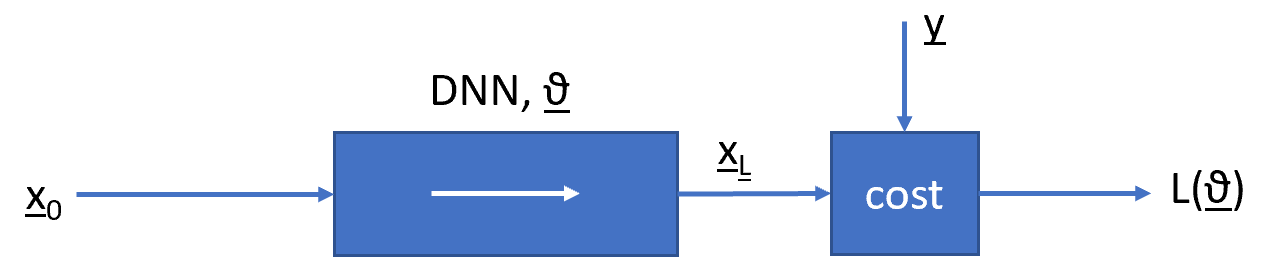
\includegraphics[width=0.45\linewidth]{Graphiken/ForwardPass_DNN}}
	\qquad
	\subfloat[Layer of Neurons compressed visualization\label{fig:BackwardPass_DNN}]{%			
		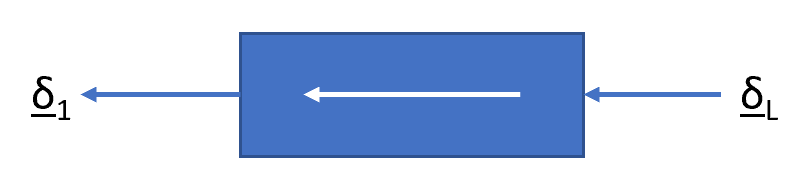
\includegraphics[width=0.45\linewidth]{Graphiken/BackwardPass_DNN}}
	\caption{Layer of Neurons in feedforward neural network}
	\label{fig:Backprop_DNN}
\end{figure}
By backpropagating through the network, $\underline{\delta}_{1}^{T}$ gives in the end the error vector of the network. This information will then be used for updating the weights and biases following an numerical optimization algorithm like the stochastic gradient descent algorithm.\\
\cite{Bishop} summarizes the error backpropagation in four steps:
\begin{enumerate}
	\item Apply the input $\underline{x}_{0}$ to the network and forward propagate through the network as in figure \ref{fig:ForwardPass_DNN} to find activations of all the hidden and output units.
	\item Evaluate the error vector $\underline{\delta}_{L}^{T}$ for all output units using equation \ref{eq:ErrorVector_OutputLayer}
	\item Backpropagate the error vectors through $\underline{\delta}_{l}^{T}$ the network following \ref{eq:ErrorVector_generalLayer} to obtain the error vector for each hidden unit in the network (figure \ref{fig:BackwardPass_DNN})
	\item Apply a numerical optimization algorithm (i.e. SGD) to adapt the network parameters
\end{enumerate}
Training (optimizing) a neural network is a difficult task and suffers from a number of optimization difficulties. Table \ref{tab:Difficulties} gives a rough summary about the difficulties and solutions in optimizing a neural network \cite{LectureNotes_DeepLearning}.\\
\begin{table}
    \centering
    \caption{Difficulties in optimizing a neural network}
    \label{tab:Difficulties}
    \begin{tabular}{lcc}
        \toprule
        Difficulty & Solutions\\
        \midrule
        stochastic gradient & larger minibatch size, momentum\\
        ill conditioning & momentum, input scaling and batch normalization\\
        saddle point / plateau & noisy gradient\\
        sensitive to step size & learning rate schedule\\
        local minimum & parameter initialization\\
        vanishing gradient & parameter initialization, improved model\\
        \bottomrule
    \end{tabular}
\end{table}
As mentioned in \cite{DeepLearningDive}, optimization provides a way to minimize the loss function for deep learning, but, in essence, the goals of optimization and deep learning are different. In pure optimization, we want to minimize the (training) loss function. But in deep learning, we focus on minimizing the generalization error, which is the value of the loss function computed on new, unseen data (test data). Thus it is important to regularly apply test data to the network while training, to see if the network is overfitted to the training data. This means, the error on the training data is very small in comparison to the test/generalization error. There are various methods to ensure overfitting does not take place, i.e. dropout or regularization (\cite{Goodfellow-et-al-2016}, \cite{Nielsen-Michael}, \cite{DeepLearningDive}, \cite{Bishop}).
\section{Unsupervised Learning}
\subsection{Dimensionality Reduction/Representation Learning}
\subsection{Clustering}
\chapter{Working Environment (Framework)}
\section{Tensorflow}
\section{Framework}
\chapter{Preliminary Architectures and Algorithm}
\section{Autoencoder}
\section{Variational Autoencoder}
\section{kMeans}
\section{Gaussian Mixture Model}
\section{IDEC}
\chapter{Experimental Setup}
\section{Datasets}
\section{Investigated Hyperparameters}
\chapter{Results}
\chapter{Summary and Outlook}

Then we include a graphic in figure \ref{mind} and information about captions in table \ref{captions}.\\
\begin{figure}
	\centering
	
\includegraphics[scale=.3]{isslogocolor}
	\caption{A beautiful mind}
	\label{mind}
\end{figure}

\begin{table}
    \centering
    \caption{Where to put the caption}
    \label{captions}
    \begin{tabular}{lcc}
         & above & below\\
        for figures & no & yes\\
        for tables & yes & no\\
    \end{tabular}
\end{table}


Lorem ipsum dolor sit amet, consetetur sadipscing elitr, sed diam nonumy eirmod tempor invidunt ut labore et dolore magna aliquyam erat, sed diam voluptua. At vero eos et accusam et justo duo dolores et ea rebum. Stet clita kasd gubergren, no sea takimata sanctus est Lorem ipsum dolor sit amet. Lorem ipsum dolor sit amet, consetetur sadipscing elitr, sed diam nonumy eirmod tempor invidunt ut labore et dolore magna aliquyam erat, sed diam voluptua. At vero eos et accusam et justo duo dolores et ea rebum. Stet clita kasd gubergren, no sea takimata sanctus est Lorem ipsum dolor sit amet.
\newpage
Lorem ipsum dolor sit amet, consetetur sadipscing elitr, sed diam nonumy eirmod tempor invidunt ut labore et dolore magna aliquyam erat, sed diam voluptua. At vero eos et accusam et justo duo dolores et ea rebum. Stet clita kasd gubergren, no sea takimata sanctus est Lorem ipsum dolor sit amet. Lorem ipsum dolor sit amet, consetetur sadipscing elitr, sed diam nonumy eirmod tempor invidunt ut labore et dolore magna aliquyam erat, sed diam voluptua. At vero eos et accusam et justo duo dolores et ea rebum. Stet clita kasd gubergren, no sea takimata sanctus est Lorem ipsum dolor sit amet.


\appendix
\chapter{Additionally}
You may do an appendix

	% -------------------> end writing here <------------------------
	% *****************************************************************
	\ifthenelse{\equal{\doclang}{german}}{
		\bibliographystyle{IEEEtran_ISSger}
	}{
		\bibliographystyle{IEEEtran_ISS}
	}
	\bibliography{refs}
	
	% *****************************************************************
	%% Additional page with Declaration ("Eidesstattliche Erklrung");
	%% completed automatically
	\begin{titlepage}
		\vfill
		\LARGE \ifthenelse{\equal{\doclang}{german}}{\textbf{Erkl\"arung}}{\textbf{Declaration}}
		\vfill
		
		\ifthenelse{\equal{\doclang}{german}}{
			Hiermit erkl\"are ich, dass ich diese Arbeit selbstst\"andig verfasst und keine anderen als die angegebenen
			Quellen und Hilfsmittel benutzt habe.
		}
		{
			Herewith, we declare that we have developed and written the enclosed thesis entirely by ourself and that I have not used sources or means except those declared.
		}
		
		\vspace{1cm}
		
		\ifthenelse{\equal{\doclang}{german}}{
			Die Arbeit wurde bisher keiner anderen Pr\"ufungsbeh\"orde vorgelegt und auch noch nicht ver\"offentlicht.
		}
		{
			This thesis has not been submitted to any other authority to achieve an academic grading and has not been published elsewhere.
		}
		
		\vfill
		
		
		Stuttgart, \signagedate
		\hfill
		\begin{tabular}{l}
			\hline
			\student
		\end{tabular}
	\end{titlepage}
	
	
	
\end{document}
